\documentclass[]{article}
\usepackage{lmodern}
\usepackage{amssymb,amsmath}
\usepackage{ifxetex,ifluatex}
\usepackage{fixltx2e} % provides \textsubscript
\ifnum 0\ifxetex 1\fi\ifluatex 1\fi=0 % if pdftex
  \usepackage[T1]{fontenc}
  \usepackage[utf8]{inputenc}
\else % if luatex or xelatex
  \ifxetex
    \usepackage{mathspec}
  \else
    \usepackage{fontspec}
  \fi
  \defaultfontfeatures{Ligatures=TeX,Scale=MatchLowercase}
\fi
% use upquote if available, for straight quotes in verbatim environments
\IfFileExists{upquote.sty}{\usepackage{upquote}}{}
% use microtype if available
\IfFileExists{microtype.sty}{%
\usepackage{microtype}
\UseMicrotypeSet[protrusion]{basicmath} % disable protrusion for tt fonts
}{}
\usepackage[margin=1in]{geometry}
\usepackage{hyperref}
\hypersetup{unicode=true,
            pdfborder={0 0 0},
            breaklinks=true}
\urlstyle{same}  % don't use monospace font for urls
\usepackage{graphicx,grffile}
\makeatletter
\def\maxwidth{\ifdim\Gin@nat@width>\linewidth\linewidth\else\Gin@nat@width\fi}
\def\maxheight{\ifdim\Gin@nat@height>\textheight\textheight\else\Gin@nat@height\fi}
\makeatother
% Scale images if necessary, so that they will not overflow the page
% margins by default, and it is still possible to overwrite the defaults
% using explicit options in \includegraphics[width, height, ...]{}
\setkeys{Gin}{width=\maxwidth,height=\maxheight,keepaspectratio}
\IfFileExists{parskip.sty}{%
\usepackage{parskip}
}{% else
\setlength{\parindent}{0pt}
\setlength{\parskip}{6pt plus 2pt minus 1pt}
}
\setlength{\emergencystretch}{3em}  % prevent overfull lines
\providecommand{\tightlist}{%
  \setlength{\itemsep}{0pt}\setlength{\parskip}{0pt}}
\setcounter{secnumdepth}{0}
% Redefines (sub)paragraphs to behave more like sections
\ifx\paragraph\undefined\else
\let\oldparagraph\paragraph
\renewcommand{\paragraph}[1]{\oldparagraph{#1}\mbox{}}
\fi
\ifx\subparagraph\undefined\else
\let\oldsubparagraph\subparagraph
\renewcommand{\subparagraph}[1]{\oldsubparagraph{#1}\mbox{}}
\fi

%%% Use protect on footnotes to avoid problems with footnotes in titles
\let\rmarkdownfootnote\footnote%
\def\footnote{\protect\rmarkdownfootnote}

%%% Change title format to be more compact
\usepackage{titling}

% Create subtitle command for use in maketitle
\providecommand{\subtitle}[1]{
  \posttitle{
    \begin{center}\large#1\end{center}
    }
}

\setlength{\droptitle}{-2em}

  \title{}
    \pretitle{\vspace{\droptitle}}
  \posttitle{}
    \author{}
    \preauthor{}\postauthor{}
    \date{}
    \predate{}\postdate{}
  

\begin{document}

\hypertarget{power-ranking-faqs}{%
\subsubsection{Power Ranking FAQs}\label{power-ranking-faqs}}

\begin{enumerate}
\def\labelenumi{\arabic{enumi}.}
\item
  \textbf{What do the rankings mean?} They attempt to rank the top
  players in Fortnite battle royale based on recent performance.The
  system uses a quantitiative model described below, but there is only
  so much you can tell from the data, and you may have issues with
  particular player rankings. Still, you will notice players with recent
  strong placements moving up, and others moving down, so it should give
  a sense of which players are worth watching.
\item
  \textbf{Which events are taken into account?} We will only be
  including major Epic events beginning with the World Cup qualifiers
  through the trio and squad Champion Series, plus whatever comes next.
  We won't be including TwitchCon or invitational events.
\item
  \textbf{How are points allocated?} Points are based on Epic's regional
  prize pool for each event. However, we do not use Epic payouts
  directly to rank players. Epic's payout tiers have steep ``steps''
  where the top placements make a lot of money,and payouts quickly drop
  off to a level where many players earn the same small payout. For
  tournaments, this makes sense, because you want to reward the very
  best performances in order to make finishing in the top slots
  especially profitable. But our aim is different: we want to aknowkedge
  consistent performance, so we take the total prize pool and ``smooth
  it out'', so everyone in an event and region makes a slightly
  different amount based on their placement.So someone who finishes \#2
  makes a little less than \#1, and someone who finishes \#50 makes a
  little less than \#49, etc.
\end{enumerate}

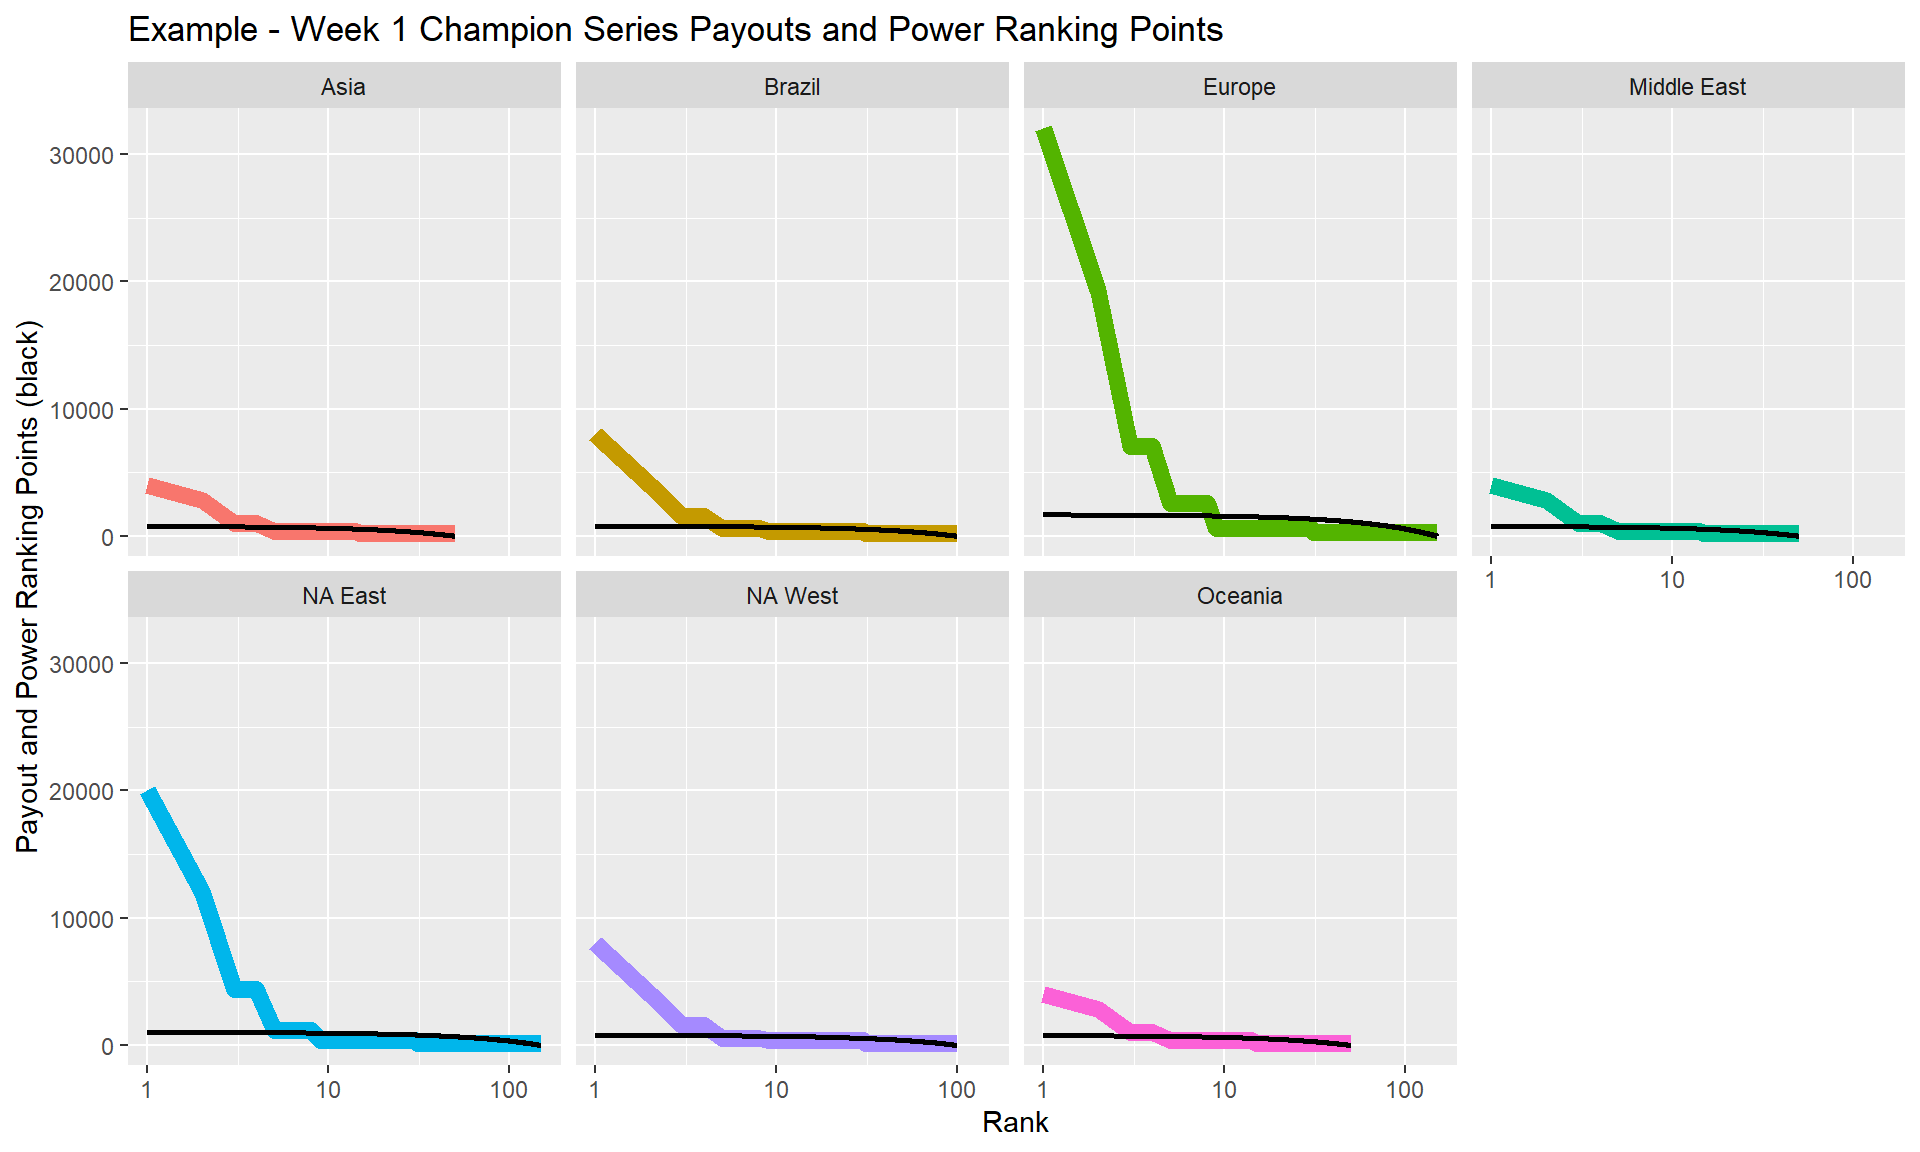
\includegraphics{Figs/power_ranking_chart-1.pdf}

\begin{enumerate}
\def\labelenumi{\arabic{enumi}.}
\setcounter{enumi}{3}
\item
  \textbf{How do the World Cup and Champion Series Finals factor in?}
  The model makes an exception for finals, since payouts for these are
  large compared to qualifiers and other Epic events. Since we don't
  want to skew the scores based on these outsized payouts, and don't
  want to penalize those who didn't qualify to much, the payouts for
  these events are divied by how much larger they are than qualifying
  events. This means that World Cup finals payouts are divided by 15 (15
  million vs 1 million), and Champion Series payouts are divided by 3 (3
  million vs 1 million.) We will use the same formula for upcoming
  events.
\item
  \textbf{Do recent events count more than past events?} Yes. In the
  model, the most recent event counts 100\%, the next less-recent counts
  98\%, etc. So an event that is 50 events ``old'' will not add anything
  to a player's power ranking. We may adjust this rule somewhat as we
  add future events to our database.
\item
  \textbf{Should I compare the rankings of players from different
  regions?} Probably not. While the same calculation method is used in
  all regions, the scores are ultimately based on how Epic allocated the
  prize pool regionally. If you believe these payouts favor some regions
  over others, you should not compare scores of players in different
  regions. Regardless, you typicaly just want to see the rankings for
  single region. To do that, click the region you want to see on the
  left to filter out the other regions.
\item
  \textbf{How do the rankings work across different formats (solo, dou,
  trio, squad?)} By default, the system combines results across all
  formats. If you want limit it to duo performance (for example), click
  only the duo events, and view the rankings. The more players involved
  in a particular team, the more difficult is is to guage the
  contribution a single player. If there is interest, we may add
  separate power rankings at the solo, duo, trio or squad level.
\item
  \textbf{Player ``x'' seems to be ranked too low (or too high.) How do
  I make sense of this?} As much as possible, we want avoid makng the
  power rankings a ``black box.'' Search for player and see their page.
  Their ``Power Points'' column for event are arrived at by multiplying
  their ``Scaled Payout'' by their ``Week Weight.'' If, looking at the
  math, something seems wrong, please DM us.\\
\item
  **When will this be updated? The aim is to update the rankings within
  a day or two of each event, via a mostly automated process. Updates
  will be tweeted at @fortniteping1
\item
  \textbf{If I see a problem who do I contact?} DM @fortniteping1
\end{enumerate}


\end{document}
